\documentclass[
	twoside=false,
	paper=a4,
	fontsize=11pt,
	parskip=half,
	ngerman
]{scrbook}

\newif\ifprintversion
\printversionfalse

\newif\ifdraft
\drafttrue

% === Page  ===
\ifprintversion
  \usepackage[
    paper=a4paper,
    % bindingoffset=10mm,
    twoside]
  {geometry}
\else 
  \usepackage[paper=a4paper]{geometry}
\fi

\ifdraft
  \usepackage{draftwatermark}
  \SetWatermarkLightness{0.8}
  \SetWatermarkText{draft/Entwurf}
  \SetWatermarkAngle{0}
  \SetWatermarkVerCenter{0.93\pdfpageheight}
  \SetWatermarkScale{0.17}
\fi

% === Fonts  ===
\DeclareUnicodeCharacter{2009}{\,} 
\usepackage{noto}
\usepackage{ebgaramond}
\usepackage[scale=0.75]{sourcecodepro}
\usepackage[cmintegrals,cmbraces]{newtxmath}
\usepackage{ebgaramond-maths}
% Redefining missing symbols
% https://tex.stackexchange.com/questions/215270/can-someone-explain-this-weird-font-behavior-ebgaramond-maths
\makeatletter
  \DeclareSymbolFont{ntxletters}{OML}{ntxmi}{m}{it}
  \SetSymbolFont{ntxletters}{bold}{OML}{ntxmi}{b}{it}
  \re@DeclareMathSymbol{\leftharpoonup}{\mathrel}{ntxletters}{"28}
  \re@DeclareMathSymbol{\leftharpoondown}{\mathrel}{ntxletters}{"29}
  \re@DeclareMathSymbol{\rightharpoonup}{\mathrel}{ntxletters}{"2A}
  \re@DeclareMathSymbol{\rightharpoondown}{\mathrel}{ntxletters}{"2B}
  \re@DeclareMathSymbol{\triangleleft}{\mathbin}{ntxletters}{"2F}
  \re@DeclareMathSymbol{\triangleright}{\mathbin}{ntxletters}{"2E}
  \re@DeclareMathSymbol{\partial}{\mathord}{ntxletters}{"40}
  \re@DeclareMathSymbol{\flat}{\mathord}{ntxletters}{"5B}
  \re@DeclareMathSymbol{\natural}{\mathord}{ntxletters}{"5C}
  \re@DeclareMathSymbol{\star}{\mathbin}{ntxletters}{"3F}
  \re@DeclareMathSymbol{\smile}{\mathrel}{ntxletters}{"5E}
  \re@DeclareMathSymbol{\frown}{\mathrel}{ntxletters}{"5F}
  \re@DeclareMathSymbol{\sharp}{\mathord}{ntxletters}{"5D}
  \re@DeclareMathAccent{\vec}{\mathord}{ntxletters}{"7E}
\makeatother
\renewcommand{\epsilon}{\varepsilon}
\usepackage[]{todonotes}


%\usepackage[osf, sc]{mathpazo}
%\linespread{1.03}
\usepackage{setspace}

\usepackage[T1]{fontenc}
\usepackage{eurosym}
\newcommand{\red}[1]{\colorbox{red}{\textcolor{white}{\textbf{#1}}}}

\addtokomafont{paragraph}{\small}
\addtokomafont{subparagraph}{\tiny}

\makeatletter
\DeclareRobustCommand{\GaUsS}{%
  G\kern-.35em
  {
    \sbox\z@ U\vbox to\ht\z@{
      \hbox{\check@mathfonts\fontsize\sf@size\z@\math@fontsfalse\selectfont A}
      \vss
    }}\kern-.15emU\kern-.1667em\lower.5ex\hbox{S}\kern-.125emS
}
\makeatother


% === Math stuff ===
\usepackage{amsmath}
\usepackage{amsfonts}
\usepackage{mathtools}
\usepackage{braket}
\usepackage[retain-explicit-plus, separate-uncertainty=true]{siunitx}
\DeclareSIUnit\gauss{G}
\sisetup{per-mode=fraction,fraction-function=\tfrac}
\usepackage{physics}
% Preventing italic variables in ket to interfere with the Ket
\newcommand{\KetSpaced}[1]{\Ket{~#1}}
\newcommand{\KetText}[1]{\Ket{\text{#1}}}

% === Tables ===
\usepackage{booktabs}
\usepackage{tabu}
\usepackage{tabularx}
\usepackage{ltablex}
\usepackage{multirow}
\usepackage{longtable}

% === Quotes  ===
\usepackage{csquotes}
\usepackage{epigraph}
\usepackage{listings}
\usepackage{xcolor}
\definecolor{stringcolor}{RGB}{154,91,145}  % rebecca
\definecolor{keywordcolor}{RGB}{80,189,233} % blue
\definecolor{commentcolor}{RGB}{255,0,0}  % red
\lstset{
  basicstyle=\ttfamily,
  numbers=left,
  breaklines=true,
  language=Python,
  otherkeywords={True,False},
  commentstyle=\color{commentcolor},
  keywordstyle=\color{keywordcolor}\bfseries,
  stringstyle=\color{stringcolor},
  emph={},
  emphstyle={\color{keywordcolor}},
}

% === Graphics ===
\usepackage{tikz}
\usepackage{subcaption}
\usepackage{pgf}
\usepackage{pgfplots}
\pgfplotsset{compat=1.11}
% \usepackage{float}
\newcommand{\imagepath}{}
\usepackage{rotating}

\definecolor{thesisred}{RGB}{255,0,0}
\definecolor{thesisgray}{RGB}{71,72,71}
\definecolor{thesisrebecca}{RGB}{105,62,163}
\definecolor{thesisfuchsia}{RGB}{154,91,145}
\definecolor{thesisblue}{RGB}{80,189,233}

% === Citations ===
\usepackage[
  %style=authoryear,
  style=apa,
  %style=numeric,
  backend=biber,
  sorting=nty,
]{biblatex}
\addbibresource{../EconBA.bib}
\PassOptionsToPackage{hyphens}{url}
\AtEveryBibitem{
  %\clearfield{urlyear}
  \clearfield{note}
  \clearfield{extra}
  \clearfield{annotation}
  \clearfield{month}
}{}


% === Glossary ===
\usepackage[acronym]{glossaries}
\makeglossaries
\newacronym{bert}{BERT}{Bidirectional Encoder Representations from Transformers}
\newacronym{lda}{LDA}{Latent Dirichlet allocation}
\newacronym{nlp}{NLP}{natural language processing}
\newacronym{pca}{PCA}{principal component analysis}
\newacronym{ses}{SES}{socioeconomic status}
\newacronym{tsne}{tSNE}{$t$-distributed stochastic neighbor embedding}


% === Title ===
\title{Idols and Socioeconomic Status}
\subtitle{Exploring Role Models using Natural Language Processing}
\newcommand{\titleDE}{Idole und sozioökonomischer Status}
\newcommand{\subtitleDE}{Eine Untersuchung von 
Vorbildern mittels Computerlinguistik}
\author{Tobias Maximilian Philipp Schattauer}
\date{February 2023}

\makeatletter
\usepackage[
	pdftitle={\@title: \@subtitle},
	pdfauthor={Tobias Maximilian Philipp Schattauer},
	pdfkeywords={}
	]{hyperref}
\makeatother

\pagenumbering{gobble}
\fontsize{10}{10}
\geometry{a4paper, margin=2cm}

\begin{document}
    \begin{center}
        \textsf{\textbf{\large{\textsc{Idols and Socioeconomic Status: Exploring Role Models using NLP}}}}\\
        Bachelor's thesis, Maximilian Schattauer, February 2023
    \end{center}


    \subsection*{Role Models \& SES}
    Both role models and SES influence child development, prosocial behavior, and education \& career.
    The influence of role models is determined by their perceived relatability and proximity (gender, ethnicity, domain).

    \textbf{$\rightarrow$ Are there interaction effects between role model perception and SES?}


    \subsection*{Data \& Methods}
    \begin{minipage}[t]{0.48\textwidth}
        \textbf{Survey Data:}
        \begin{itemize}
            \item 13- and 14-years-old adolescents interviewed about role models (245 from low-, 96 from high-SES backgrounds)
            \item 184 valid celebriry role models named
        \end{itemize}
    \end{minipage}
    \hspace{0.04\textwidth}
    \begin{minipage}[t]{0.48\textwidth}
        \textbf{Online Newspaper Articles:}
        \begin{itemize}
            \item about adolescents' role models
            \item preprocessed and balanced per role model
        \end{itemize}
    \end{minipage}

    \vspace{0.2cm}
    \begin{minipage}[t]{0.48\textwidth}
        \textbf{Topic Modelling:} Finding dominant topics among the articles and assigning each article a topic probabilistically.
        \begin{center}
            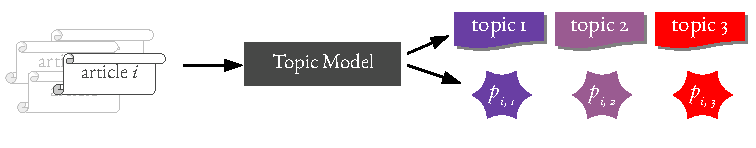
\includegraphics[width=\textwidth]{img/topic_modelling_schema_simple.pdf}
        \end{center}
    \end{minipage}
    \hspace{0.04\textwidth}
    \begin{minipage}[t]{0.48\textwidth}
        \textbf{Zero-Shot Classification:} Assiging to each article a label from a predefined set of labels, able of capturing connotations.
        \begin{center}
            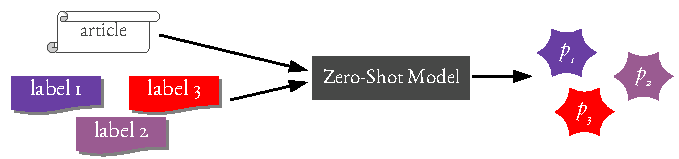
\includegraphics[width=\textwidth]{img/zero_shot_schema_simple.pdf}
        \end{center}
    \end{minipage}

    \subsection*{Findings}
    \begin{center}
        \begin{minipage}[t]{0.22\textwidth}
            \small{\textbf{Topics:} low SES: sports and music more common, high SES: movie more common}

            \resizebox{!}{\textwidth}{../../presentation/img/semantic_clustering_hypertopic_distribution_distinct.pgf}
        \end{minipage}
        \hspace{0.03\textwidth}
        \begin{minipage}[t]{0.22\textwidth}
            \small{\textbf{Sentiment}: positive correlation between SES and sentiment}

            \resizebox{!}{\textwidth}{../../presentation/img/zero_shot_distribution_sentiment_n_distinct.pgf}
        \end{minipage}
        \hspace{0.03\textwidth}
        \begin{minipage}[t]{0.22\textwidth}
            \small{\textbf{Prosociality}: positive correlation between SES and prosocial connotations}

            \resizebox{!}{\textwidth}{../../../build/thesis/70-supervised/zero_shot_distribution_prosociality_distinct.pgf}
        \end{minipage}
        \hspace{0.03\textwidth}
        \begin{minipage}[t]{0.22\textwidth}
            \small{\textbf{Crime}: significantly more drug connotation in low-SES group}

            \resizebox{!}{\textwidth}{../../presentation/img/zero_shot_distribution_crime_type_distinct.pgf}
        \end{minipage}
    \end{center}

    \subsection*{Validity \& Improvements}
    \begin{itemize}
        \item potential threat: limited data abundance and variety, too few times each role models was mentions $\rightarrow$ include social media data, increase survey mentions per role model
        \item naive aggregation strategy: only examining distribution of articles $\rightarrow$ aggregate per role model and identify interesting role models
        \item model tuning $\rightarrow$ label articles to fine-tune models
    \end{itemize}
\end{document}